\documentclass[12pt]{report}

% Document Structure and Formatting
\usepackage[a4paper, margin=1in]{geometry} % Set paper size and margins
\usepackage{setspace}  % Line spacing
% \onehalfspacing        % Set line spacing to 1.5 (recommended for theses)
\doublespacing
\usepackage{indentfirst} % Indent the first paragraph of each section
\usepackage{titlesec}  % Customize section headings
% \titlespacing*{\chapter}{0pt}{0pt}{10pt} % Removes line break
% \titleformat{\chapter}[hang]{\normalfont\huge\bfseries}{\thechapter}{1em}{} % Title format
\usepackage{ragged2e}  % Enables text justification
% \usepackage[colorinlistoftodos]{todonotes}
\usepackage{amssymb}
\usepackage{pifont}

% Mycrotype allows for character protusion ox XeLaTeX.
\usepackage[stretch=20]{microtype}
% It has more features, but those are only supported on other compilers

\usepackage{geometry} % Required for adjusting page dimensions and margins
\geometry{
	paper=a4paper, % Paper size
	top=2.5cm, % Top margin
	bottom=3cm, % Bottom margin
	left=2.5cm, % Left margin
	right=2.5cm, % Right margin
	headheight=14pt, % Header height
	footskip=1.5cm, % Space from the bottom margin to the baseline of the footer
	headsep=1.2cm, % Space from the top margin to the baseline of the header
	% showframe, % Uncomment to show how the type block is set on the page
}

\usepackage{xargs}  % Use more than one optional parameter in a new commands
\usepackage[
	backgroundcolor=white,
	bordercolor=red, % try white!
	linecolor=red,
	figcolor=white,
	figwidth=.8\textwidth,
	tickmarkheight=.8em,
	textwidth=20mm,
	obeyFinal
]{todonotes}
\setlength{\marginparwidth}{20mm}

% Usage: \mytodo{something to go on the margin}
\newcommandx{\mytodo}[2][1=]{\todo[size=tiny,#1]{\begin{spacing}{0.5}#2\end{spacing}}}
\newcommandx{\prof}[2][1=]{\todo[linecolor=gray,bordercolor=gray,size=tiny,#1]{\begin{spacing}{0.5}#2\end{spacing}}}
\newcommandx{\duvida}[2][1=]{\todo[linecolor=blue,bordercolor=blue,size=tiny,#1]{\begin{spacing}{0.5}#2\end{spacing}}}
% Usage:
% \todoin{
%   Inline text much as an env.
% }
\newcommand\todoin[2][]{\vspace{1em} \todo[inline,noprepend,caption={} #1]{#2}}


% Language and Fonts
\usepackage[T1]{fontenc}   % Better font encoding
\usepackage[utf8]{inputenc} % Allow UTF-8 characters (e.g., accents)
% \usepackage{lmodern}       % Modern font
% \usepackage{microtype}     % Improves text spacing and justification
\usepackage[brazil]{babel} % ou [portuguese]

\newcount\XeTeXtracingfonts % Remove some debug info chatter

%% XCharter
% \usepackage[scale=0.96]{XCharter} % Use the XCharter text font

%% Libertine
\usepackage{libertine}
% \usepackage{libertinust1math}
% \usepackage[libertine]{newtxmath} % Set the math font

%% Libertinus (more modern fork of libertine)
% \usepackage{libertinus}

%% Fix DOI font
% \renewcommand\UrlFont{\rmfamily}

%% Other math font
% \usepackage[bitstream-charter]{mathdesign}

%% TextTT font
\usepackage[scaled=1.05,proportional,lightcondensed]{zlmtt}


% Images and Graphics
\usepackage{graphicx}  % Include images
\usepackage{float}     % Control image positioning
\usepackage{subcaption} % Subfigures
\usepackage{tikz}
\usetikzlibrary{positioning, arrows}

% Tables
\usepackage{booktabs}   % Professional-looking tables
\usepackage{longtable}  % Multi-page tables
\usepackage{array}      % Custom column formatting
\usepackage{multirow}

% Math symbols
\usepackage{amsmath, amssymb, amsthm}  % Mathematical symbols & environments
\usepackage{mathtools}  % Extended math features
\allowdisplaybreaks  
% \usepackage{mathrsfs}

% Lists and References
\usepackage{enumitem}  % Customizable lists
\usepackage{hyperref}  % Clickable links
\usepackage[nameinlink,noabbrev]{cleveref}
% Tradução dos nomes dos ambientes
\crefname{equation}{Equação}{Equações}
\Crefname{equation}{Equação}{Equações}
\crefname{chapter}{Seção}{Seções}
\Crefname{chapter}{Seção}{Seções}

% Forçar conjunções em português
\makeatletter
\def\creflastconjunction{ e~}
\def\crefmiddleconjunction{,~}
\def\crefrangeconjunction{--}
\makeatother

% Bibliography
\usepackage[
	backend=biber,
	style=numeric,
	sorting=none,
	maxnames=99,
	minnames=1,
	maxcitenames=2,    % mostra no máximo 2 autores na citação
	mincitenames=1     % usa "et al." a partir de 3 autores
]{biblatex}
\addbibresource{references.bib}


% Custom commands
\newcommand{\R}{\mathbb{R}}  % Example: shorthand for real numbers
\renewcommand{\thetable}{\arabic{table}} % Continuous enumeration for tables
\renewcommand{\thefigure}{\arabic{figure}} % Continuous enumeration for figures

\makeatletter
\renewcommand{\theequation}{\arabic{equation}}
\makeatother

\usepackage{chngcntr}
\counterwithout{equation}{chapter} % já está usando
\counterwithout{figure}{chapter}   % mantém contagem contínua de figuras
\counterwithout{table}{chapter}    % mantém contagem contínua de tabelas

% Comando para comentar inline
\newcommand{\comentario}[1]{}

  % Loads packages and custom commands

\begin{document}

\begin{titlepage}
    \centering

    {\Large UNICAMP - Instituto de Computação \par}
    {\Large MO420 - Programação Linear Inteira \par}

    \vspace{0.5cm}

    {\Large \textbf{Trabalho Final} \par}
    {\Large \textbf{Explorando Abordagens para o Trigger Arc Traveling Salesperson Problem} \par}
    \vspace{1cm}

    {\Large \textbf{Aluno:} Vitor Antônio Pimenta Silva \par}
    \vspace{0.5cm}

    {\Large \textbf{Professor:} Prof. Dr. Flávio Keidi Miyazawa \par}
    \vspace{0.7cm}

    {\Large \textbf{Resumo} \par}  
    \vspace{0.5cm}

    \begin{flushleft}
        \justifying
        Neste trabalho foram abordadas diferentes técnicas para produzir limitantes superiores e inferiores para o \emph{Trigger Arc Traveling Salesperson Problem} (TATSP). Nesta variante do TSP o objetivo é minimizar os custos de um ciclo hamiltoniano porém com a adição de efeitos dinâmicos sobre as arestas. Por se tratar de um TSP com restrições adicionais, é um problema NP-Difícil e, portanto, abordagens alternativas serão exploradas para contornar a complexidade do modelo. Foram elaboradas soluções para o programa linear inteiro (ILP) baseando-se em um modelo matemático de um trabalho prévio e, ao todo, foram desenvolvidas: uma abordagem de solução direta do ILP, utilizando o Gurobi; uma solução via Relaxação Lagrangiana (RL); e uma metaheurística \emph{Simulated Annealing} baseada na relaxação linear e em fixação de variáveis via operadores.
    \end{flushleft}
 
    \vfill
    {\Large Julho, 2025 \par}
\end{titlepage}

% \titleformat{\chapter}[hang]{\normalfont\huge\bfseries}{\thechapter}{1em}{} %

\titlespacing*{\chapter}{0pt}{0pt}{10pt} % Removes line break
\titleformat{\chapter}[hang]  % Customizes chapter titles
  {\huge\bfseries}  % Font style (huge, bold)
  {\thechapter}  % Shows only the chapter number (without "Chapter")
  {1em}  % Space between number and title
  {}  % Additional formatting (empty in this case)

% Chapters
\chapter{Descrição do Problema}
\label{chap:problem_description}

\noindent No trabalho de \textcite{Carmine2024} o TATSP foi descrito como sendo uma variante do TSP original, sendo descrito, basicamente, como um problema para encontrar um ciclo Hamiltoniano de custo mínimo em um grafo direcionado onde existem relacionamentos entre arcos. Esses relacionamentos são responsáveis por dinamizar os custos de arestas no grafo. De agora em diante referenciamos estes relacionamentos utilizando as expressões de "gatilho" ou "\emph{trigger}" para arcos (ou arestas) que ativam alteração de custo para arestas "alvo" ou "\emph{target}". O modelo matemático proposto por \textcite{Carmine2024} servirá como base de referência para nosso modelo de programação linear inteira mista.

No trabalho de \textcite{Carmine2024} é fornecido um exemplo explicativo para representar o impacto da existência de relacionamentos entre as arestas do grafo. Além disso, na competição \emph{MESS2024} \mytodo{adicionar referência aos slides da competição} também foram apresentados exemplos de casos de uso reais onde o TATSP é aplicável, ilustrando um depósito de estantes móveis, onde os arcos simulam as movimentações das estantes e os relacionamentos exploram como determinadas movimentações podem afetar os custos de movimentação de estantes no futuro.

Formalmente, em um grafo direcionado (e não necessariamente completo) $G = (N, A)$, onde $N$ é o conjunto de vértices ou nós e $A$ é o conjunto de arcos ou arestas direcionados. O objetivo é determinar um ciclo Hamiltoniano de custo mínimo considerando a existência de relacionamentos entre as arestas definidos como $r = (t, a)$, significando que o custo da aresta $a$ será alterado caso a aresta $t$ seja escolhida para o caminho e esteja \textbf{antes} de $a$ na ordem de visitação.

Seja $c(a) \in R^{+} \forall a \in A$ o custo de passar pelo arco $a$. Para cada arco $a = (h,k)$ existe um conjunto de relacionamentos $R_a = \{(a_1, a) | a_1 \in A\}$ representando todos os relacionamentos que afetam o arco $a$. Além disso, define-se $c(r) \in R^{+} \forall r \in R_a$ como os novos custos para o arco $a$ caso a relação $r$ esteja \textbf{ativa}. Além disso, definimos $R$ como sendo o conjunto de todos os relacionamentos (para todos os arcos) da instância. Considerando essas entradas, utilizamos, integralmente, o modelo matemático de \textcite{Carmine2024}, descrito a seguir.

São quatro conjuntos de variáveis de decisão binárias e um conjunto de variáveis inteiras auxiliar, sendo definidos como:

\begin{itemize}
    \item \textbf{$x_a$}: binárias com valor $1$ quando o arco $a$ está presente no caminho, e $0$ caso contrário. Estas variáveis indicam quais arcos estarão no caminho construído.
    \item \textbf{$y_a$}: binárias com valor $1$ quando não há relacionamento ativo em $R_a$ e $x_a=1$, e $0$ caso contrário.
    \item \textbf{$y_r$}: binárias com valor $1$ quando o relacionamento $r$ está ativo, e $0$ caso contrário.
    \item \textbf{$y^{hat}_{r}$}: binárias com valor $1$ quando, para uma relação $r = (a_1, a)$, o arco $a$ precede o arco $a_1$ no caminho, e $0$ caso contrário.
    \item \textbf{$u$}: inteiras utilizadas como auxiliares para definir a ordem de visitação de cada nó do grafo. Esta variável é importante para as restrições que evitam a existência de subciclos na solução.
\end{itemize}

Assim, a formulação completa segue:

\vspace{-2em}
\begin{align}
    \text{(TATSP)} \quad & \min Z = \sum_{r \in R} c(r)y_r + \sum_{a \in A} c(a)y_a \label{eq:funcao_objetivo} \\[4pt]
    \text{sujeito a} \notag \\[2pt]
    & \sum_{(i,j) \in A} x_{ij} = |N| & \quad & \label{eq:C1} \\[2pt]
    & u_i + 1 \leq u_j + M(1 - x_{ij}) & \quad & \forall (i,j) \in A/j \neq 0 \label{eq:C2}  \\[2pt]
    & \sum_{(i,j) \in A} x_{ij} = 1 & \quad & \forall j \in N \label{eq:C3} \\[2pt]
    & \sum_{(i,j) \in A} x_{ij} = 1 & \quad & \forall i \in N \label{eq:C4} \\[2pt]
    & y_a + \sum_{r \in R_a} y_r = x_{ij} & \quad & \forall a = (i,j) \in A \label{eq:C5} \\[2pt]
    & y_r \leq x_{ij} & \quad & \forall r=((i,j), (h,k)) \in R \label{eq:C6} \\[2pt]
    & u_i + 1 \leq u_h + M(1 - y_r) & \quad & \forall r=((i,j), (h,k)) \in R \label{eq:C7} \\[2pt]
    & u_h + 1 \leq u_i + M(1 - \hat{y}_{r}) & \quad & \forall r=((i,j), (h,k)) \in R  \label{eq:C8} \\[2pt]
    & x_{ij} \leq (1 - x_{hk}) + (1 - y_{hk}) + \hat{y}_{r} & \quad & \forall r=((i,j), (h,k)) \in R \label{eq:C9} \\[2pt]
    & u_{\hat{i}} - M(\hat{y}_{r2}) \leq u_i + M(2 - y_{r1} - x_{\hat{i}\hat{j}}) - 1 & \quad &
    \begin{aligned}[t]
        & \forall r1=((i,j), (h,k)) \in R, \\
        & \forall r2=((\hat{i},\hat{j}), (h,k)) \in R
    \end{aligned} \label{eq:C10} \\[2pt]
    & x_{ij}, y_a \in \{0, 1\} & \quad & \forall a=(i,j) \in A \label{eq:C11} \\[2pt]
    & y_r, \hat{y}_{r} \in \{0,1\} & \quad & \forall r \in R \label{eq:C12} \\[2pt]
    & u_i \in \{0,|N|\} & \quad & \forall i \in N \label{eq:C13}
\end{align}

Começando pela \cref{eq:funcao_objetivo}, temos o objetivo de minimizar o custo do caminho. Cada um dos termos indica se o custo de cada arco do caminho será o custo base (original) ou o custo modificado por um relacionamento. A \cref{eq:C1}, referida no código como restrição $C1$, é responsável por garantir que o número de arcos do caminho seja igual à quantidade de nós da entrada, sendo uma condição mínima para o ciclo Hamiltoniano. A \cref{eq:C2} controla a posição dos vértices, servindo de auxílio para conferir a ordem de visitação do caminho, além de garantir que não existam subciclos. Já as \crefrange{eq:C3}{eq:C4} garantem que cada nó tenha apenas um arco de entrada e outro de saída, além de também tornarem a \cref{eq:C1} redundante e desnecessária ao modelo. As restrições da \cref{eq:C5} são responsáveis por garantir que somente um custo pode ser associado a um arco (seja o modificado, o base ou zero). Em seguida, a \cref{eq:C6} produz restrições que requerem que a relação $r=((i,j), (h,k))$ esteja ativa se o caminho passar pelo arco gatilho $(i,j)$. A \cref{eq:C7} garantem o controle de precedência entre os gatilhos e alvos, ou seja, se o arco gatilho $(i,j)$ não precede o alvo $(h,k)$, então $y_r = 0$. Já a \cref{eq:C8} visa garantir que, se o arco $(h,k)$ não precede $(i,j)$ na solução, então $\hat{y}_r = 0$. A restrição descrita pela \cref{eq:C9} trabalha com diferentes condições para cada $r=((i,j), (h,k)) \in R$, onde o arco gatilho $(i,j)$ só pode ser usado se o arco $(h,k)$ não é usado; ou se a variável $y_{hk}$ associada ao custo base do arco $(h,k)$ não está ativa; ou se ambos os arcos $(i,j)$ e $(h,k)$ são usados na solução, $(i,j)$ aparece após $(h,k)$. E, por fim, o conjunto de restrições da \cref{eq:C10} define uma relação de precedência entre os relacionamentos, garantindo que um arco alvo $(h,k)$ tenha seu custo alterado pelo arco gatilho mais recente (mas ainda anterior a ele). As restrições dadas pelas \crefrange{eq:C11}{eq:C13} indicam os tipos das variáveis utilizadas.

\chapter{Métodos}
\label{chap:methodology}

\noindent Nesta seção trataremos sobre as abordagens utilizadas no desenvolvimento do trabalho. Foram feitas implementações para três opções de ataque ao TATSP: Programação Linear Inteira (ILP), Relaxação Lagrangiana (RL) e uma metaheurística \emph{Simulated Annealing} baseada na relaxação linear (SA).

\section{Programação Linear Inteira -- ILP}
\noindent A primeira abordagem a ser codificada foi a de programação linear inteira, utilizando o modelo matemático base \cite{Carmine2025} e resolvendo o problema com o \emph{solver} comercial Gurobi. A ideia principal foi de tentar alcançar soluções exatas para as instâncias do problema. Matematicamente, o modelo é suficiente para produzir soluções ótimas, porém, a realidade da execução é que a medida em que as instâncias crescem, a complexidade computacional associada ao problema também cresce, principalmente em problemas de natureza combinatória \cite{Wolsey2020}.

Utilizando a linguagem de programação Julia e os pacotes JuMP, Gurobi, dentre outros utilitários, foi codificada uma solução baseada no modelo matemático TATSP, porém adicionando uma restrição para garantir que a primeira posição do caminho fosse ocupada pelo vértice $1$ (1-indexado) que, em termos práticos, seria o vértice que representa o "depósito". No código foi chamada de "C0" e é da forma $u[1] = 1$.

\section{Relaxação Lagrangiana -- RL}
\noindent Percebendo a dificuldade de convergir para uma solução, a segunda abordagem utiliza a Relaxação Lagrangiana como base para produzir limitantes superiores e inferiores. A ideia por trás disso é produzir limitantes de maneira iterativa para tentar reduzir o \emph{gap} aproximando-se ao valor ótimo. O limitante inferior, chamado de \emph{lower bound}, vem de uma solução produzida após dualizar restrições consideradas problemáticas (geralmente restrições que estendem o modelo e o tornam mais complexo, por exemplo). Basicamente essas restrições passam a ser termos de penalização na função objetivo e seus pesos são dados por multiplicadores de Lagrange. Em seguida, com essa solução (não necessariamente viável), pode-se utilizar diferentes técnicas para produzir um limitante superior (\emph{upper bound}), que indica uma solução viável para o problema original mas que não necessariamente é ótima.

Para o TATSP, foi codificada uma versão que se aproveita do ILP e usa alguns artifícios para modularizar a dualização de restrições. A ideia por trás disso foi ser capaz de explorar quais restrições poderiam beneficiar a relaxação e também a viabilização para a construção de um \emph{upper bound}. A implementação foi feita baseada no material de aula e no livro de \textcite{Bertsimas1998}.

Para o TATSP, dualizar as restrições $C6 - C10$ (\crefrange{eq:C6}{eq:C10}), reduz o problema, praticamente, a um TSP. Mesmo que ainda seja um problema NP-Difícil, para chamadas iterativas ao \emph{solver}, isso já representa uma redução de complexidade. Além disso, ao dualizar as restrições relacionadas somente aos gatilhos, pode-se garantir que o \emph{Gurobi} irá produzir caminhos viáveis, sendo assim, para construir um \emph{upper bound} basta, após a otimização, recomputar os custos reais dos arcos a partir do caminho feito. Porém, é importante reconhecer que para instâncias maiores, resolver o TSP por si só já é muito desafiador.

A cada iteração é computada a violação de cada restrição dualizada e são atualizados os multiplicadores de Lagrange para ela. Além disso, a cada iteração é recalculado o passo utilizando o valor da função objetivo com o melhor \emph{upper bound} encontrado até o momento (\emph{Polyak}). Isso é importante para ajudar na convergência do método do subgradiente.

No capítulo de experimentos são mostrados os resultados de exploração das diferentes dualizações.

\section{Metaheurística Simulated Annealing -- SA}

Além da relaxação Lagrangiana, foi desenvolvida uma heurística baseada na técnica de Simulated Annealing (SA) aplicada sobre a relaxação linear (LP) do modelo exato do TATSP. Essa abordagem visa explorar o espaço de soluções fracionárias da LP para obter boas soluções inteiras viáveis, construindo assim limites superiores de qualidade para o problema.

A ideia central consiste em relaxar a integridade das variáveis binárias do modelo original (ILP), permitindo que assumam valores contínuos entre 0 e 1. A solução da LP contêm valores fracionários para as variáveis de decisão $x_a$ e $y_r$, os quais serão utilzados como "guias probabilísticos" para a construção de soluções inteiras (\emph{upper bounds}). No entanto, essas soluções fracionárias não necessariamente satisfazem, todas as restrições do TATSP, especialmente aquelas relacionadas à ativação condicional dos arcos. Para isso, empregamos uma estratégia de viabilização baseada em fixações progressivas das variáveis de ativação $y_r$.

A ideia de utilizar o SA partiu de uma curiosidade de exploração e após ver alguns trabalhos que utilizavam essa metaheurística para problemas de variantes baseadas no TSP. Porém, foi mais comum encontrar o SA inserido em híbridos mais complexos. Aqui, foi utilizado o SA puro visando também explorar a abordagem para um problema relativamente novo (introduzido em 2025 por \textcite{Carmine2025}) na literatura.

O algoritmo proposto visa utilizar os mecanismos de exploração do SA para aplicar fixações sucessivas às variáveis $y_r$ a cada iteração. São utilizados três operadores para definir o critério de fixação das variáveis e, além disso, o modelo relaxado é modificado para que $x_a$ e $u$ retomem suas características de binárias e inteiras, respectivamente. A intenção por trás disso é reduzir o problema por meio da fixação de variáveis ligadas aos gatilhos (que se mostraram ordens de grandeza mais impactantes nas instâncias) mas ainda ser capaz de usar a solução do solver como um caminho viável. Dessa forma, a cada iteração é possível produzir um \emph{upper bound} em tempo polinomial $O(NTriggers*NArcs)$ no pior caso.

A cada iteração a busca realizada escolhe, aleatoriamente uma estratégia de fixação dentre as três implementadas. Essas estratégias se baseiam num sistema de pontuação para os gatilhos. Essa pontuação é construída a partir do peso do arco na relaxação linear ($x_a$) e na diferença entre o custo base do arco alvo e seu custo modificado após ter o gatilho ativado. Sendo assim, os operadores disponíveis tem políticas próprias que definem quais gatilhos $y_r$ serão zerados por possuir um \emph{score} considerado ruim.

O primeiro operador é o \emph{topk} que seleciona uma fração definida ($20\%$, por exemplo) das piores pontuações encontradas para ser fixada em zero. O segundo é o \emph{weighted} que atribui pesos aos gatilhos e coleta uma fração definida deles para fixar. E o terceiro é o \emph{threshold} que basicamente olha para os valores das variáveis fracionárias $y_r$ na relaxação e busca aqueles que superam um determinado valor (\emph{threshold}) para serem fixados.

Em seguida, após aplicar o operador, o novo modelo é enviado ao \emph{solver} e resolvido, produzindo um caminho viável porém com um custo distorcido. Para tanto é utilizado um método que recomputa o valor da função objetivo para atender ao problema original, produzindo assim um limitante superior válido.

E, seguindo o fluxo do \emph{Simulated Annealing}, é utilizado o critério de Metropolis \cite{Gendreau2010} para definir o aceite do novo limitante como sendo o melhor. Ao inserir uma probabilidade de aceitar soluções piores, é possível sair de eventuais ótimos locais e explorar melhor o espaço de solução.

Essa heurística de viabilização baseada em SA pode ser promissora, visto que permite um controle mais refinado da complexidade computacional e por aproveitar o custo informativo do LP relaxado. Sua flexibilidade permite adaptações tanto na definição dos operadores quanto nas estratégias de resfriamento, viabilizando uma busca balanceada entre exploração e intensificação\cite{Gendreau2010}.

Por fim, vale destacar a importância de um refinamento na calibração dos parâmetros, tanto da Relaxação Lagrangiana quanto da metaheurística do \emph{Simulated Annealing}.

\chapter{Experimentos Computacionais}
\label{chap:experiments}

\noindent Com o problema delineado, um modelo matemático pronto (TATSP) e três abordagens distintas implementadas, seguimos para a seção de experimentos visando avaliar o desempenho de cada ideia proposta.

Para realizar os experimentos foi utilizado um ambiente Ubuntu $22.04$, com $16$GB de RAM e um processador Intel Core $i7-12700H$ de $2.30$ GHz. Além disso o \emph{solver} escolhido foi o \emph{Gurobi} sob uma licença acadêmica e a linguagem de programação utilizada para implementar as abordagens foi Julia na versão $1.11$.

Os experimentos realizados se utilizam de instâncias fornecidas na competição MESS2024~\cite{MESS2024}. Dada a extensa lista de instâncias, foram selecionadas três instâncias de cada grupo, totalizando 6 instâncias, sendo duas consideradas pequenas, duas médias e duas grandes. Para cada uma delas foram testados os algoritmos.

Para as instâncias menores, é possível notar que ambos os algoritmos conseguiram explorar o espaço de busca. Para a Relaxação Lagrangiana em ambos os casos (\autoref{fig:grf101_RL} e \autoref{fig:grf1_RL}) houve uma parada antes do número de iterações estipulado. Isso foi uma regra adicional para interromper a execução caso se passassem $30\%$ do total de iterações sem haver melhoras em quaisquer limitantes. Porém é interessante notar que há uma flutuação no decorrer da execução.

\begin{figure}[H]
    \centering
    \begin{minipage}{0.48\textwidth}
        \centering
        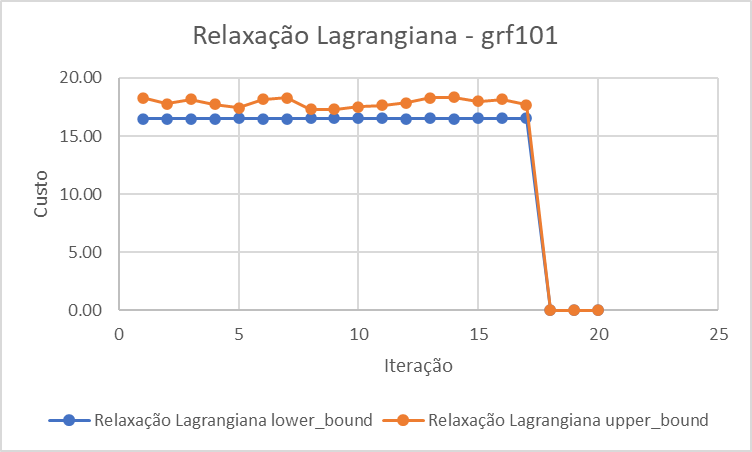
\includegraphics[width=\linewidth]{./images/grf101_RL.png}
        \caption{Relaxação Lagrangiana - grf101}
        \label{fig:grf101_RL}
    \end{minipage}
    \hfill
    \begin{minipage}{0.48\textwidth}
        \centering
        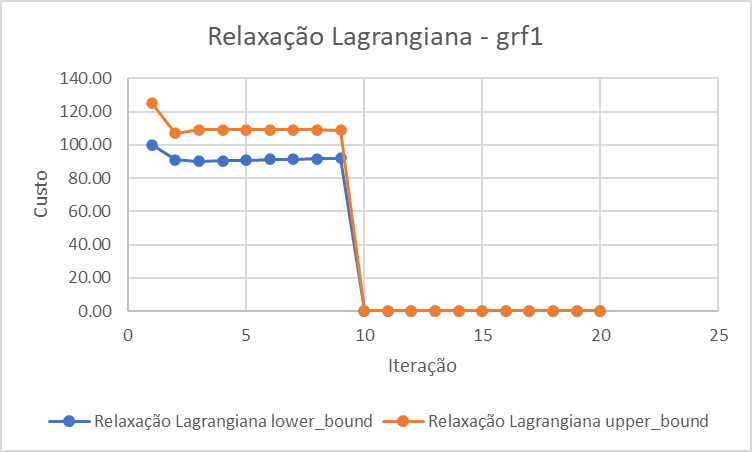
\includegraphics[width=\linewidth]{./images/grf1_RL.png}
        \caption{Simulated Annealing - grf101}
        \label{fig:grf101_SA}
    \end{minipage}
\end{figure}

Para o caso do \emph{Simulated Annealing} (\autoref{fig:grf101_SA} e \autoref{fig:grf1_SA}), notam-se picos na execução do algoritmo ao longo das iterações, o que é um comportamento esperado para essa metaheurística. A parametrização, apesar de básica, conseguiu gerar diversidade nas soluções e, de certa forma, explorar as possibilidades. No que diz respeito ao uso de tempo, para as instâncias pequenas, o tempo limite de $10$ minutos para cada uma foi suficiente para execução total de cada passo. Para \emph{grf101} a RL utilizou $515.0$ segundos e para o SA $339.0$ segundos. Já para a \emph{grf1}, a RL utilizou $279.0$ segundos (\emph{early stop} citado anteriormente) e para o SA $605.0$ segundos.

\begin{figure}[H]
    \centering
    \begin{minipage}{0.48\textwidth}
        \centering
        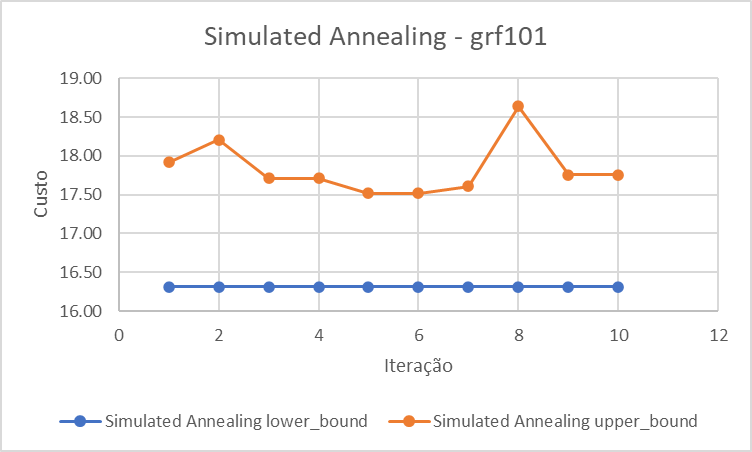
\includegraphics[width=\linewidth]{./images/grf101_SA.png}
        \caption{Relaxação Lagrangiana - grf1}
        \label{fig:grf1_RL}
    \end{minipage}
    \hfill
    \begin{minipage}{0.48\textwidth}
        \centering
        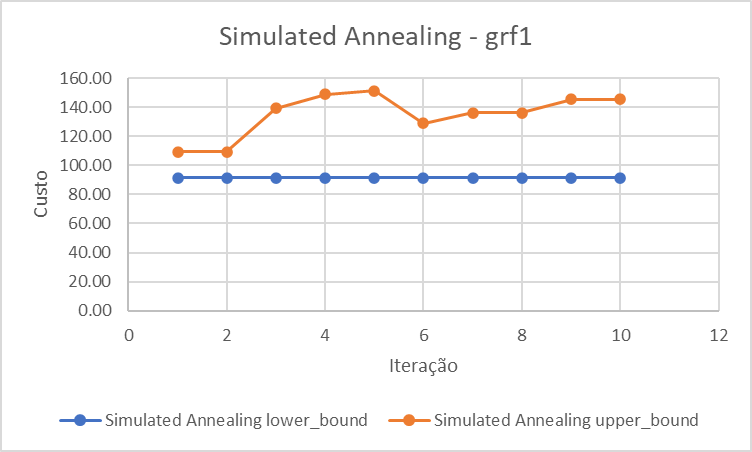
\includegraphics[width=\linewidth]{./images/grf1_SA.png}
        \caption{Simulated Annealing - grf1}
        \label{fig:grf1_SA}
    \end{minipage}
\end{figure}

Para as instâncias médias e grandes selecionadas, \emph{grf8, grf112, grf18 e grf129}, infelizmente, foram encontradas barreiras com relação ao uso de memória para a execução tanto da Relaxação Lagrangiana, pois o número de gatilhos estoura a memória para o vetor de violações, especialmente para a restrição $C10$; e também para o SA, pois o modelo continua grande demais para o tempo limite dividido entre as iterações, atingindo $60$ segundos ainda durante a fase de \emph{pre-solve} do Gurobi.

Porém, para o ILP foi possível construir os modelos inteiros e iniciar a otimização, como mostra a \autoref{tab:resultados-tatsp-ilp}. Apesar de não atingir \emph{gaps} razoáveis para os casos em questão, foi ao menos possível obter uma solução viável, exceto para a instância \emph{grf129}. E, Com exceção à instância \emph{grf101}, considerada a menor, todas as outras atingiram o tempo limite sem alcançar valores ótimos. Apesar disso, para as instâncias menores, foi possível notar que os limitantes alcançados são representativos para os valores encontrados pelo \emph{solver}, ou seja, limitam superior e inferiormente o ótimo do problema original.


\begin{table}[H]
\centering
\begin{tabular}{|c|c|c|}
\hline
\textbf{Instâncias} & \textbf{Custo} & \textbf{Status} \\
\hline
grf101 & 16.94   & OPTIMAL      \\
grf1   & 101.70  & TIME\_LIMIT   \\
grf112 & 50.93   & TIME\_LIMIT   \\
grf8   & 223.43  & TIME\_LIMIT   \\
grf129 & 0.00    & OUT\_OF\_MEMORY \\
grf18  & 355.55  & TIME\_LIMIT   \\
\hline
\end{tabular}
\caption{ILP para as seis instâncias.}
\label{tab:resultados-tatsp-ilp}
\end{table}

Por último, foi realizado um experimento focado na instância \emph{grf101} visando observar o desempenho da Relaxação Lagrangiana para diferentes dualizações das restrições de gatilhos. A \autoref{tab:dualizacao-limits} mostra como a dualização de restrições afeta os resultados mesmo em instâncias pequenas. A medida em que aumentamos o número de restrições dualizadas, nota-se uma piora na produção de limitantes, tanto inferiores quanto superiores. A queda mais brusca está ligada à restrição C10, tanto em tempo quanto qualidade. A suspeita mais forte é de que esse seja um conjunto de restrições muito grande, por ser construído aos pares de gatilhos, dois a dois. Além disso, isso afeta mais ainda a penalização da função objetivo.

\begin{table}[H]
\centering
\begin{tabular}{|c|c|c|c|c|c|c|c|}
\hline
\textbf{C6} & \textbf{C7} & \textbf{C8} & \textbf{C9} & \textbf{C10} & \textbf{Lower Bound} & \textbf{Upper Bound} & \textbf{Time(s)} \\
\hline
\checkmark & \ding{55} & \ding{55} & \ding{55} & \ding{55} & 16.53 & 17.32 & 515.0\\
\checkmark & \ding{55} & \ding{55} & \checkmark & \ding{55} & 16.51 & 17.32 & 606.0\\
\checkmark & \ding{55} & \ding{55} & \checkmark & \checkmark & 16.42 & 17.75 & 98.0\\
\checkmark & \checkmark & \checkmark & \checkmark & \checkmark & 16.30 & 17.57 & 5.0\\
\hline
\end{tabular}
\caption{Impacto da dualização progressiva das restrições C6-C10 sobre os limitantes inferior e superior.}
\label{tab:dualizacao-limits}
\end{table}

E, por último, vale citar que, ao dualizar restrições que contém \emph{Big M}, é notável a queda no tempo de execução, porém também nota-se uma flutuação expressivamente maior nos valores das violações, gerando problemas até de grandeza quando não controlados.
\chapter{Conclusões}
\label{chap:final_remarks}

\noindent Neste projeto foi feito um trabalho de exploração de um problema recente e aplicação de métodos vistos ao longo da disciplina de Programação Linear Inteira. Foi possível ainda experimentar uma linguagem de programação nova e voltada à otimização e também experimentar heurísticas diferentes.

Para o método de fixação de variáveis ainda há espaço para explorar mais tipos de fixações e também de operadores, além disso, buscar métodos mais eficazes para viabilizar soluções na parte de relaxação Lagrangiana também é uma alternativa. Mesmo que durante todos os testes a impressão mais forte que ficou é que a Relaxação Lagrangiana talvez não seja um método muito adequado para este problema, ou que pelo menos ainda existem mais possibilidades de dualizações a serem exploradas. Por último, talvez também seja interessante aliar as propostas atuais ao \emph{Concorde TSP solver}\cite{ConcordeTSPSolver}, que é reconhecido na literatura como extremamente eficiente para o TSP -- mesmo que seja para o TSP simétrico, é possível adaptar o processamento das entradas para encaixar com as necessidades dele. 

Com as implementações realizadas e após os experimentos, nota-se que ainda há muito espaço para melhora, tanto no uso de recursos quanto na parametrização dos algoritmos desenvolvidos. Apesar disso, é importante destacar o nível de discussão produzido ao atacar um problema novo. Adicionando uma nota pessoal: tive a oportunidade de discutir extensamente com os colegas sobre as abordagens, as limitações e dificuldades. Com essa rede de apoio foi possível, em um prazo relativamente curto, superar barreiras de conhecimento tanto teórico quanto técnico.

\printbibliography

% Customize references title
% \bibliography{references}


\end{document}
